\section{Ion Beam Analysis}
\textbf{a)} To identify the unkown elemental compostitions of the film, substrate and beam, the \textit{Potku} \cite{potku}. By plotting the Energy as a function of Time-of-Flight (ToF), several elemental traces are visually apparent. It is possible to add 2D gates to delimit the edges of the traces in \textit{Potku}. The program can then perform a calibration if the gates and beam are labeled correctly. 

For this, a preliminary analysis of the shape of the plot has to be done. A hypothesis of the compositions can be developed from that. If the hypothesis is correct, the calibration will be linear and all point will lie on the calibration line. 

For the initial hypothesis, the strongest traces can be identified as the film. Since the only possible film compositions are \ce{Al_2O_3} and \ce{AlN}, we know that the more massive of these traces has to correspond to aluminium. By knowing that more massive atoms have a longer ToF, we can identify the strong trace on the right (the trace that has the highest energies) as the aluminium trace. All traces to the left of this one correspond to atoms which are lighter than it. 

There is only one trace to the right of this one, and the bottom of the trace is thicker, which indicates that there is an unresolved second trace next to it. Since a substrate candidate is silicon, the neighbouring element to aluminium, we can take it for the preliminary hypothesis, ruling out germanium. 

There is still a heavier atom than aluminium and silicon in the spectrum, so fluorine can be ruled out as a beam component. Due to the distance to the last trace, we can take the heaviest possible beam component, Cu, for the hypothesis.

Finally, the traces to the left of the aluminium-tagged one have to be identified. Due to the structure seen, and knowing that the only candidates for these are nitrogen and oxygen as part of the film, the three-trace structure reveals that this must be nitrogen with some carbon and oxygen contamination. If the central, strong trace were oxygen, the slightly higher mass trace would have to be fluorine or neon contamination, which is unlikely.

Therefore, the discussed traces are identified as such in \textit{Potku}, with the areas shown in \autoref{fig:tof} as discussed. The resulting calibration plot is shown in \autoref{fig:calib}.

\begin{figure}[ht]
    \centering
    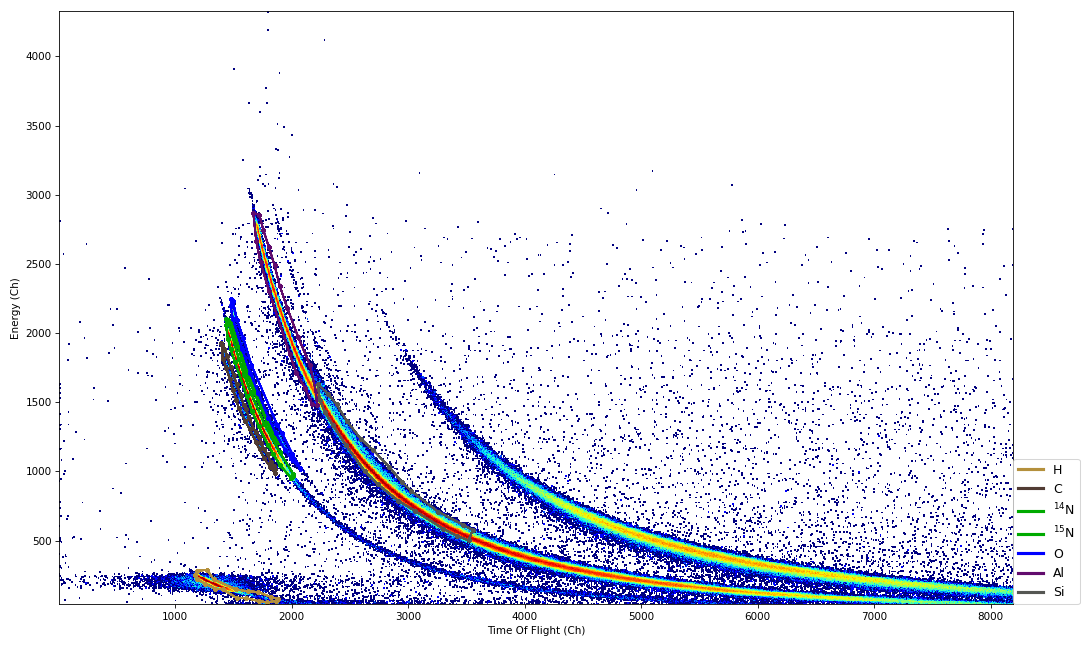
\includegraphics[width=1\textwidth]{ToF-E.png}
    \caption{Energy to Time of Flight diagram for the whole dataset, including gates for several elemental traces.}
    \label{fig:tof}
\end{figure}

\begin{figure}[ht]
    \centering
    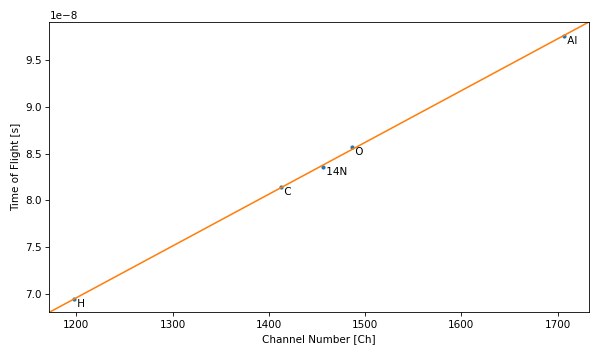
\includegraphics[width=\textwidth]{ToF-E_Calibration.png}
    \caption{Linear calibration performed by Potku, all points being on the line indicate that the elemental traces were tagged correctly.}
    \label{fig:calib}
\end{figure}